\section{Introduction}

%Introduction to 802.11ah and all the decisions left open in the standard; potential parameters to study to optimize various performance metrics.

The \gls{iot} aims to provide connectivity among tens of billions of battery powered smart devices anytime and anywhere. Currently, there are two categories of low-power IoT communication technologies: \gls{wpan} and \gls{lpwan} technologies. However, as the transmission range of the WPAN technologies is too short (i.e., tens of meters) and throughput of the LPWAN technologies is too low (i.e., up to at most a few kilobits per
second), both of them can only be applied in a limited set of IoT scenarios. 

The new IEEE 802.11ah Wi-Fi standard, marketed as Wi-Fi HaLow, fills this gap.
It operates in the unlicensed sub-1 GHz frequency bands , and support transmission ranges from 100 m up to 1 km with data rates between 0.15 Mbps and 346.67 Mbps. Thus, IEEE 802.11ah has the potential to achieve much higher
transmission ranges than existing \gls{wpan} and much higher throughput than both \gls{wpan} and \gls{lpwan}
technologies. 

On the \gls{mac} layer, a novel channel access method, referred to as \gls{raw} is proposed to provide scalable
connectivity among large number of battery powered devices. \gls{raw} is based on station grouping and attempts to
reduce contention and collisions in highly dense deployments by dividing stations into groups and allowing channel access to one group at a time. Consequently, IEEE 802.11ah allows up to 8192 stations to connect to a single Access Point (AP). Figure \ref{fig:RAW} schematically depicts how \gls{raw} works. Specifically, the channel airtime is split into several intervals, some of which are assigned to RAW groups, while others are shared and can be accessed by all stations using the traditional \gls{edca}. Moreover, each RAW group consists of one or more equal-duration slots, among which the stations assigned to the RAW group are evenly split (using round robin assignment). The \gls{raw} related information is carried in the \gls{rps} element and broadcast by \gls{ap} at fixed interval. The \gls{rps} specifies the stations belonging to each group, the group start time, slot number and slot duration. For a more in-depth description of IEEE8 02.11ah and RAW, the reader is referred to existing literature ~\cite{Khorov2015a,Sensor2017, sensors80211ah}.

\begin{figure}[t]
  \centering
  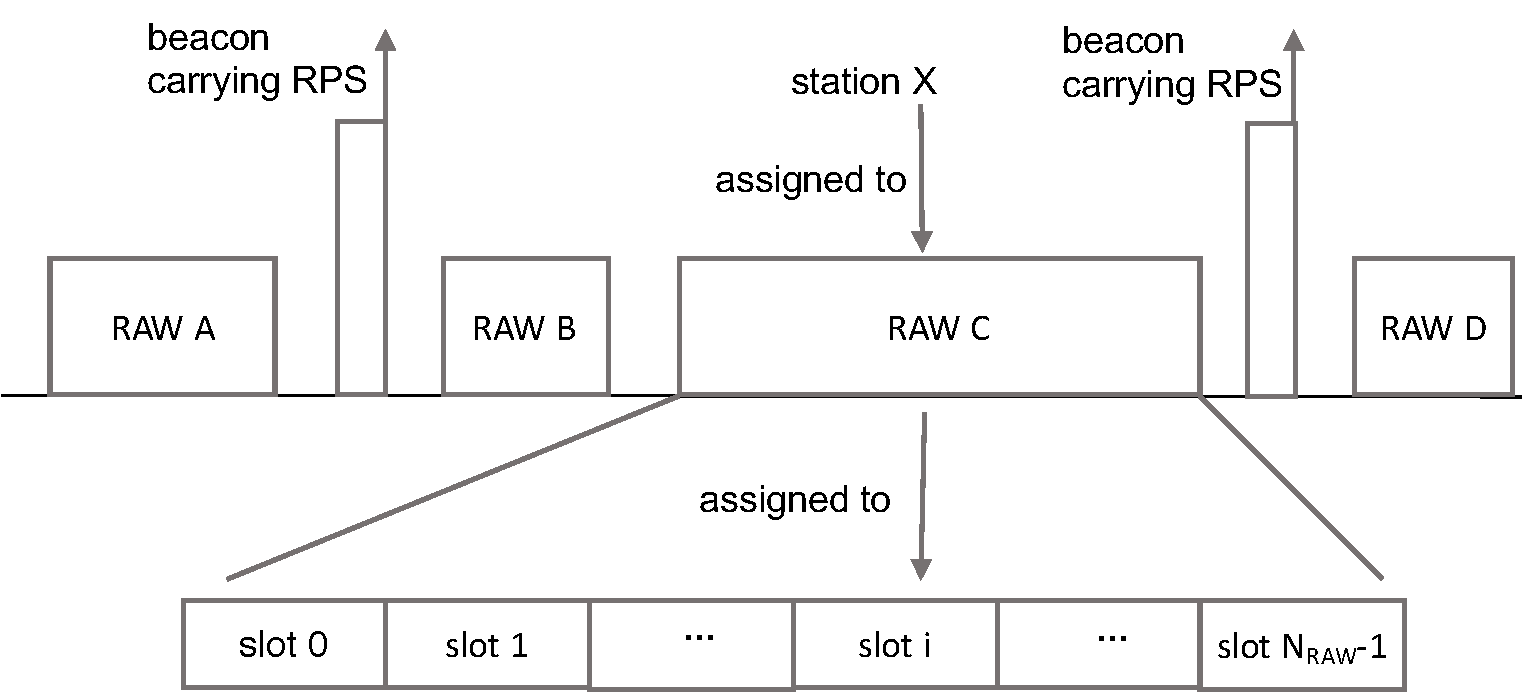
\includegraphics[width=0.8\columnwidth]{image/raw.pdf}
  \caption{\textbf{Schematic representation of the \gls{raw} mechanism}\label{fig:RAW}}
\end{figure}

The 802.11ah standard, however, does not specify how to configure the actual \gls{raw} grouping parameters. Previous research ~\cite{WoWMoM2016} has shown that the optimal \gls{raw} configuration depends on network-related parameters, such as the number of stations, traffic patterns, and network load~\cite{WoWMoM2016}. Incorrect configuration severely impacts throughput, latency and energy efficiency. However, it assumes homogeneous networks, i.e., all stations uses same \gls{mcs} and packet size, and stations are evenly divided into RAW groups. Moreover, some network-related parameters, such as beacon interval, channel width, station transmission queue size are not considered as fixed. At last but not least, many \gls{iot} applications require mobility support. Therefore, it is crucial to understand the effect of movement on performance (e.g., throughput, energy) in order to optimally configure the network.




As a step forward, in this paper, we evaluate the \gls{raw} performance with 19 network-related parameters, and use locating arrays to determine which parameters play a significant role in \gls{raw} optimization in terms of throughput and latency. In comparison to the research outlined above, the work presented in this paper is novel is two ways. First, it conducts a very comprehensive analysis on \gls{raw} performance, covering a quite broad range of network-related parameters, the obtained results can be considered as a guideline for designing \gls{raw} optimization algorithm for a variety of networks. Seconds, instead of analysis the network-related parameters exhaustively which requires \textcolor{red}{todo} experiments, the number of experiments is significant reduced by using locating arrays, only 304 (\textcolor{red}{todo\%}) experiments are used to study the \gls{raw} performance.

The remainder of this paper is structured as follows. Section~\ref{sec:parameters_selection} describes the evaluated network-related parameters and the selection of values for each parameter. 
Section~\ref{sec:locating_arrays} details the locating arrays method, how they are used for screening, and the new grouping idea to cope with the large number of values for some parameters. The experiments are described in Section~\ref{sec:setup}. Section~\ref{sec:evaluation} analysis the experiment results using locating arrays, determining the parameters which have significant roles in \gls{raw} optimization.
Finally, Section~\ref{sec:conclusion} offers conclusions and a short overview of future work.



% These works prove the strong
% correlation between network and traffic conditions on one
% hand, and the optimal RAW configuration on the other. This
% supports the hypothesis that there is a need for real-time RAW
% parameter optimization.

%evaluates \gls{raw} performance with all stations using same \gls{mcs} and packet size, the results

% In the past, several analytic models have been proposed to predict \gls{raw} performance~\cite{Khorov2015b,Wang2015}, and some algorithms has been proposed for RAW optimization~\cite{Chang2015,Ogawa2013, Qutab-Ud-Din2015, Sensor2017,Sensys2017, WoWMoM2018}. However, only a few network parameters are considered as variables. 




% As such, there is a need for \gls{raw} optimization algorithms that collect network-related information, and at the start of each beacon interval adapt the \gls{raw} configuration based on the current network conditions. 

% This is achieved using some sort model of the environment, which takes as input network conditions and a \gls{raw} configuration, and generates as output one or more performance metrics (e.g., throughput or energy consumption).



